\clearpage
\fancyhead[R]{\sffamily\small\color{Muted}Vulkan / 性能实测}
\section{摄影棚天光的烘焙与显示}
\setlength{\parindent}{2\ccwd}

摄影棚全景里有一排很亮的灯箱。移走 Stanford Bunny 场景中所有灯光，灯箱仍会从天空照亮地面。初版里，兔子左前方的地面有几块发白。换一种计算天光的方法后，同一位置的明暗过渡平缓了许多。

\begin{figure}[H]\centering
\panelimage{.485\linewidth}{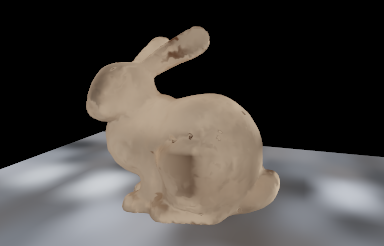
\includegraphics[width=\linewidth]{../../../output/validation/sky-probes/bunny-first.png}}{初版 · 向随机方向读取天光}
\hfill
\panelimage{.485\linewidth}{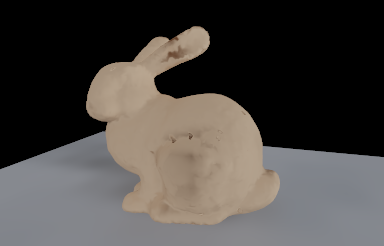
\includegraphics[width=\linewidth]{../../../output/validation/sky-probes/bunny-after.png}}{新版 · 分块累加天光，再检查遮挡}
\caption{Redflag Forge 的 Vulkan 场景面板。RenderDoc 1.47 分别回放第 24 帧，输出为 $384\times246$ 像素。相机、材质和摄影棚全景相同。}
\end{figure}

探针是房间中用来记录附近光照的采样点。初版从各个探针发出射线。有些射线刚好遇到灯箱，另一些全落在较暗的背景上，相邻两支探针的亮度就会相差很多。新版将天空立方体的每个面分成 $16\times16$ 块，先累加每块里的像素，再沿每块的代表方向检查遮挡。灯箱占的面积再小，其像素也会计入所在块。若窗框刚好切过一块，块内哪些方向可见仍是近似。

为了单独检查亮度，把模型换成无遮挡的黑色平面，保留摄影棚全景。按同一天空图直接积分，朝上的红通道应为 0.827。初版 504 支探针的读数从 0.086 到 6.537，新版全部为 0.828。把红、绿、蓝三通道都与独立积分比较，均方根误差由 0.60249 降到 0.00060。这些都是线性光照值，尚未调曝光或转换成显示器颜色。

\readings{\href{run:../validation/sky-probes/flat-first.json}{初版的平面读数}\quad
\href{run:../validation/sky-probes/flat-filtered.json}{新版及独立积分}\quad
\href{run:../../tests/check_sky_viewport.py}{编辑器机位与截帧脚本}}

\clearpage
\subsection{等待烘焙与读取探针的时间}

在已烘焙的房间里转动镜头，显卡从相邻探针读取光照，就能给新看到的地面着色。更换天光后才需要重新烘焙。前者关系到每一帧，后者关系到修改场景后要等多久。这里分别测了两种操作。

{\smalltable\noindent\begin{tabularx}{\linewidth}{@{}Xrr@{}}\toprule
测量范围 & 随机方向 & 分块积分\\\midrule
启动烘焙到进程退出，中位数（秒） & 1.987 & 1.960\\
烘焙时间，中间八成样本（秒） & 1.943--2.048 & 1.907--1.994\\
画面读取探针，GPU 中位数（微秒） & 13.072 & 12.656\\
读取探针，中间八成样本（微秒） & 12.53--13.39 & 12.37--12.87\\\bottomrule
\end{tabularx}\par}

两版都用 Windows Debug/x64 的正式 Forge 程序，在同一台 Ryzen 9 8945HX、RTX 5070 Ti Laptop GPU 电脑上运行。使用相同的兔子、底座和天空图，开启多次漫反射与 Vulkan 验证层。计时期间关闭 RenderDoc 截帧。先各预热两次，再交替运行十对，每对交换先后顺序，每次都从没有探针文件开始。

从启动 \code{--bake-probes} 到进程退出，计时包括设备初始化、读取场景、GPU 计算和写盘。两版每次写出的文件均为 96,792 字节。中位数相差 27 毫秒，小于这批样本自身的波动。要知道分块积分本身占了多少时间，还需要在烘焙命令内给相应的 GPU 指令单独计时。

随后重新打开两版兔子场景，在相同的第 24 帧截帧。事件列表里，第 68 项从探针网格插值得到每个像素的照明。两帧均没有更新探针。回放按“初版、新版、新版、初版”的顺序打开帧文件，每次先预热一次，再用 GPU 计数器读九次该事件，每版共 18 个读数。两版都在约 13 微秒完成插值，表中的数据只覆盖这个事件。

\readings{从仓库根目录运行 \href{run:../../tests/benchmark_sky_bake.py}{\nolinkurl{tests/benchmark_sky_bake.py}}，以 \code{--first}、\code{--revised} 和 \code{--scene} 指定两版程序和场景。\href{run:../../tests/replay_sky_cost.py}{RenderDoc 回放脚本}\quad
\href{run:../validation/sky-probes/bake-timing.json}{逐次等待时间}\quad
\href{run:../validation/sky-probes/gpu-first.json}{初版 GPU 读数}\quad
\href{run:../validation/sky-probes/gpu-after.json}{新版 GPU 读数}}
